\documentclass[18pt]{beamer}

\usepackage[utf8]{inputenc}
\usepackage{default}
\usepackage{graphicx}
\usepackage{amsmath}
\usepackage{amsthm}
\usepackage{amsfonts}
\usepackage{amssymb}
\usepackage{tikz}
\usetikzlibrary{tikzmark,decorations.pathreplacing}
\usefonttheme{professionalfonts}

\usetheme{Warsaw}

\beamertemplatenavigationsymbolsempty
\addtobeamertemplate{navigation symbols}{}{%
    \usebeamerfont{footline}%
    \usebeamercolor[fg]{footline}%
    \hspace{1em}%
    \insertframenumber/\inserttotalframenumber
}

\useoutertheme{smoothbars}
\useinnertheme[shadow=true]{rounded}
\usecolortheme{whale}



%\newtheorem{definition}{Definition}
\begin{document}

\title{Formalisation of the Delaunay triangulation}
\author[Clément Sartori]{Clément Sartori\\ Under the supervision of Yves Bertot}
\date{June 14, 2017}
\begin{frame}
 \maketitle
 \end{frame}


\section{Introduction}

\subsection{Triangulations}
\begin{frame}{Applications}
 Delaunay triangulations have lots of applications:
 \begin{itemize}
  \item<1,2,3,4> Terrain generation.
  \item<2,3,4> Modelise cellular coverage maps.
  \item<3,4> {\bf Path planning:}
  
  Use of Delaunay triangulations algorithms in mission-critical software for autonomous vehicles.
 \end{itemize}
\onslide<4>
 
Continuation of a previous work by Yves Bertot and Jean-Francois Dufourd, in a more abstract way.

\end{frame}

\begin{frame}{Definition}

 A triangulation $T$ of a subset $X$ of $\mathbb{R}^2$ is a tiling of this subset with triangles such
that:
\begin{itemize}
 \item<2-> The intersection of two distinct triangles is either empty or a common edge of these triangles.
 \item<3-> The union of the triangles of $T$ is $X$ itself.
\end{itemize}

\begin{overprint}
\onslide<4>
\begin{figure}
  \centering
  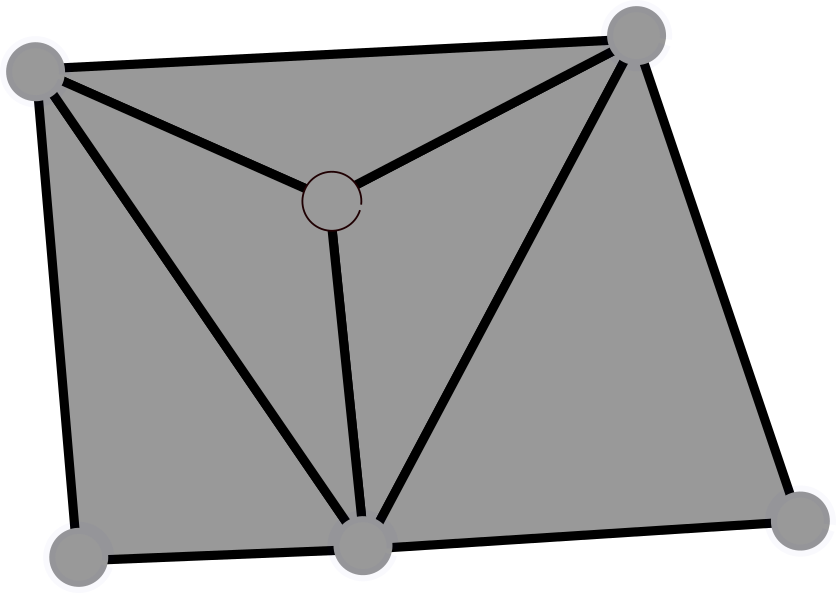
\includegraphics[scale=1.5]{Trig1}
  \caption{\label{Trig1} This is a triangulation of the convex hull of the points.}
\end{figure}

\onslide<5>
\begin{figure}
  \centering
  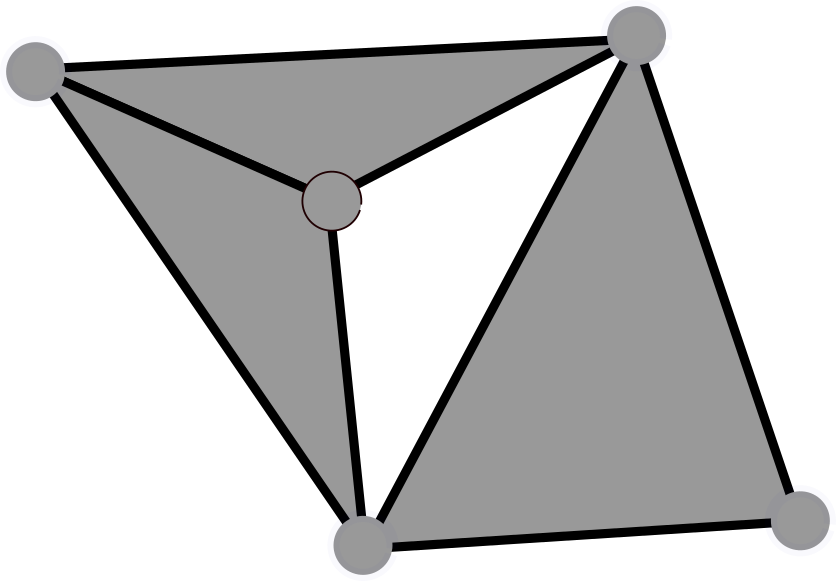
\includegraphics[scale=1.5]{NotTrig1}
  \caption{\label{NotTrig1} This is not a triangulation of the convex hull of the points.}
\end{figure}

\onslide<6>
\begin{figure}
  \centering
  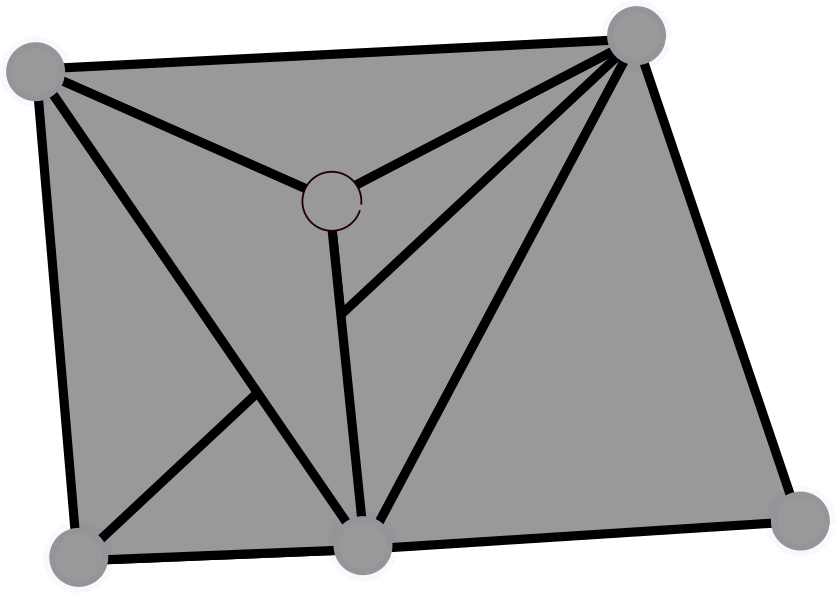
\includegraphics[scale=1.5]{NotTrig2}
  \caption{\label{NotTrig1} This is not a triangulation of the convex hull of the points.}
\end{figure}
\end{overprint}
\end{frame}

\begin{frame}{Delaunay triangulations}
 
 \begin{definition}
  A triangulation $T$ of the convex hull of a set of points $D$ is said to be a Delaunay triangulation if no point of $D$ is in the circumcircle of a triangle of $T$.
 \end{definition}
 \begin{uncoverenv}<2->
Intuitively, a Delaunay triangulation maximises the smallest angle of every triangles.
\end{uncoverenv}
 \begin{figure}

\begin{minipage}{.5\textwidth}
 \centering
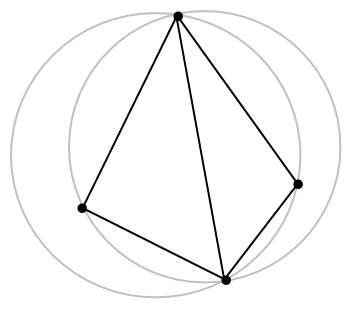
\includegraphics[scale=0.45]{Delaunay_before_flip}
\end{minipage}%
\begin{minipage}{.5\textwidth}
 \centering
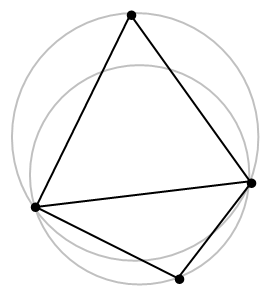
\includegraphics[scale=0.45]{Delaunay_after_flip}
\end{minipage}
\end{figure}
\end{frame}




\section{The Algorithm}

\begin{frame}{Computing Delaunay triangulations}
There is an incremental algorithm capable of computing a Delaunay triangulation of the convex hull of a set of point.

Given an existing triangulation and a point, the algorithm consists in:
\begin{enumerate}
\item<1-> Adding the point to the existing triangulation.
\item<2-> Flipping the illegal edges to obtain a Delaunay triangulation.
\end{enumerate}
\end{frame}


\subsection{Adding Points}

\begin{frame}{Adding points to a triangulation}
Three cases:

\begin{enumerate}
\item<1-> The new point is in the interior of a triangle of the triangulation.
\item<2-> The new point is on an edge of a triangle of the triangulation.
\item<3-> The new point is not in the convex hull of the existing triangulation.
\end{enumerate}

\begin{overprint}
  \onslide<1>
  \begin{figure}
\centering
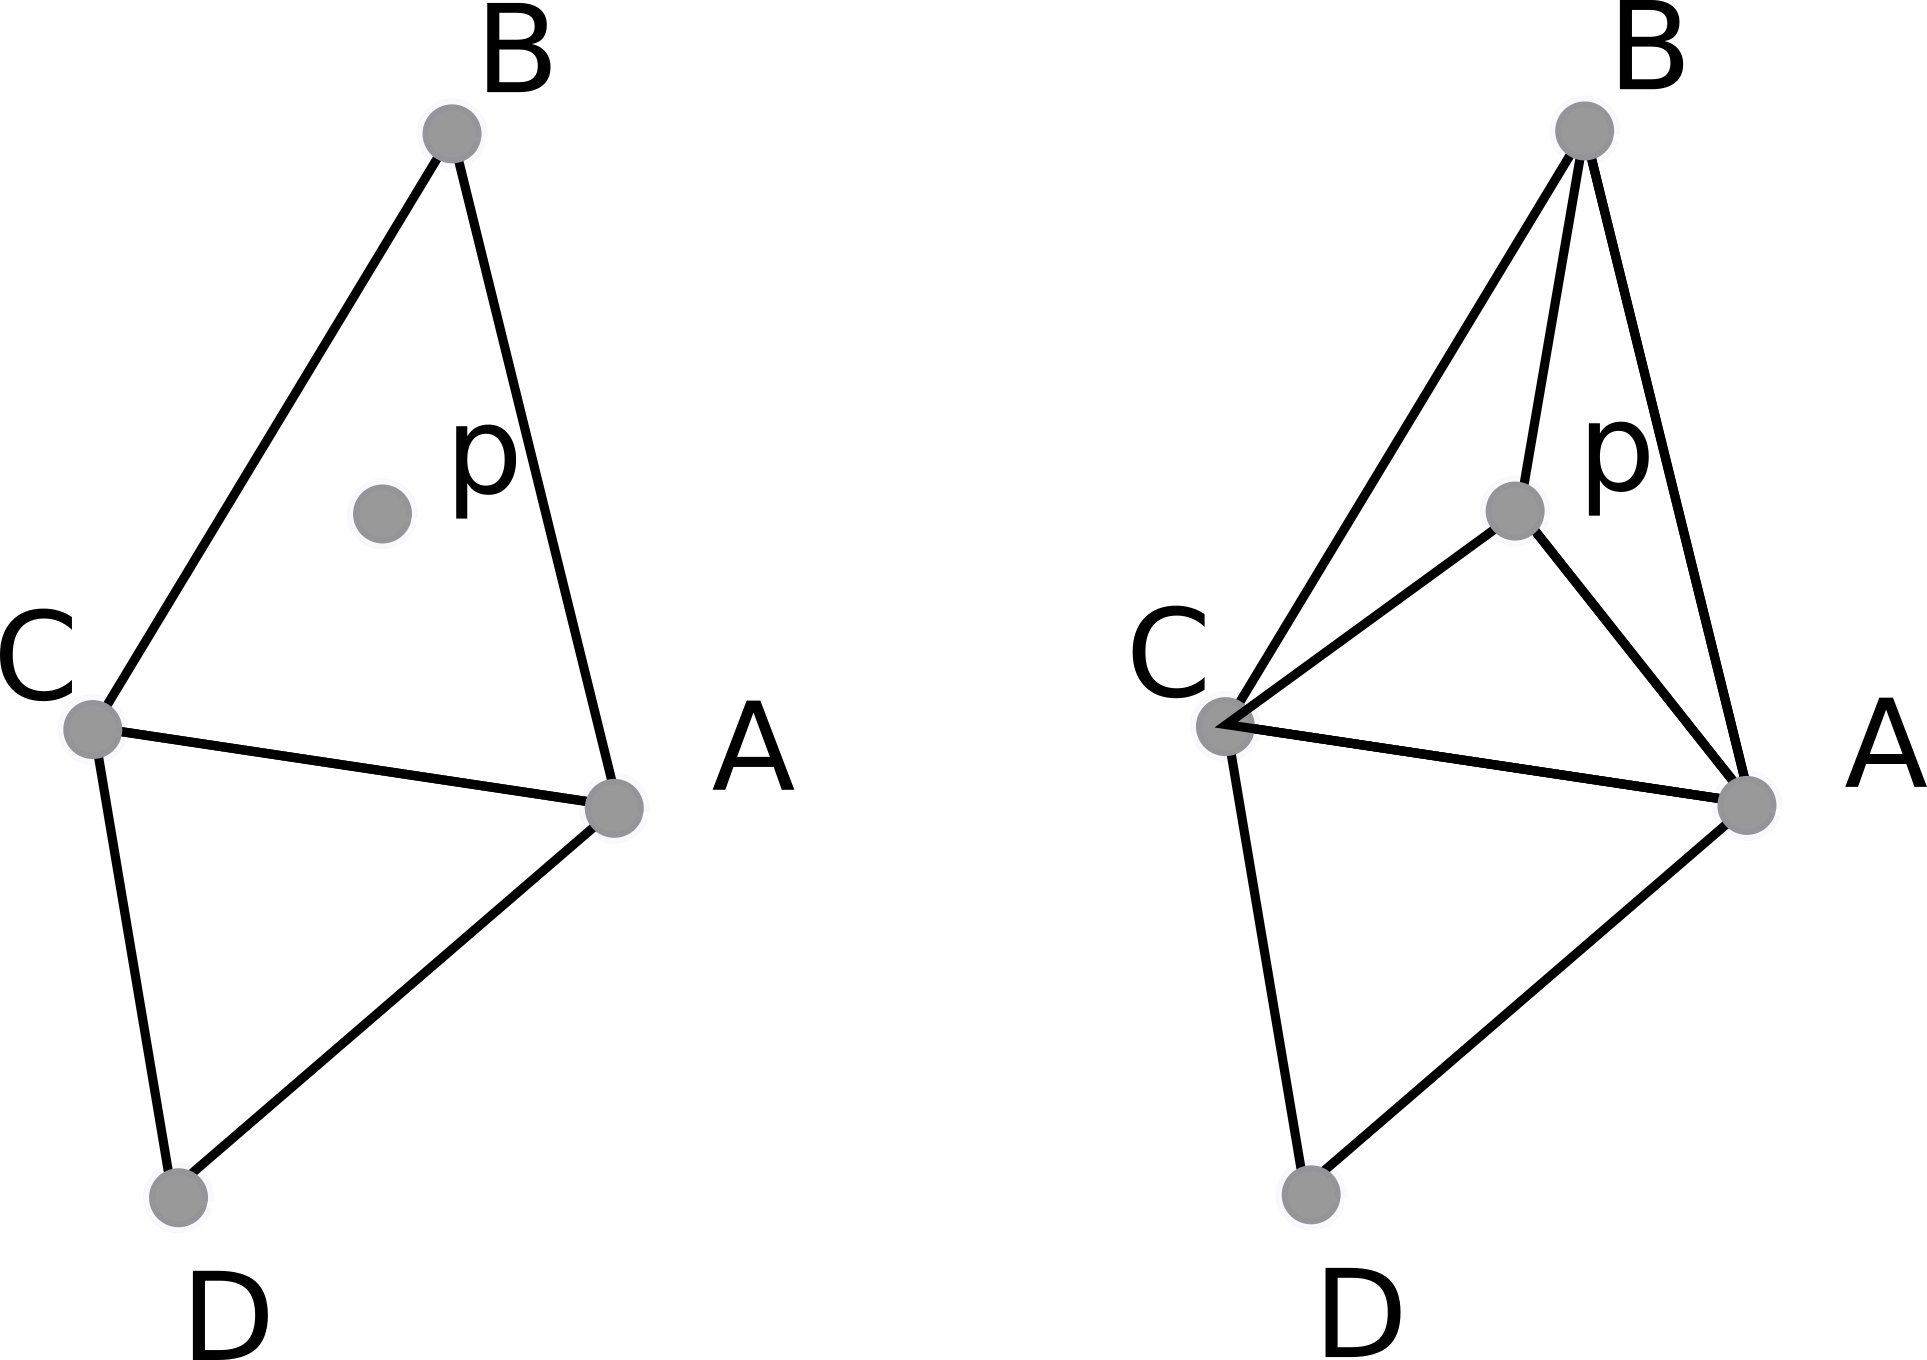
\includegraphics[scale=0.8]{adding}
\end{figure}
  \onslide<2>
  
  \begin{figure}
\centering
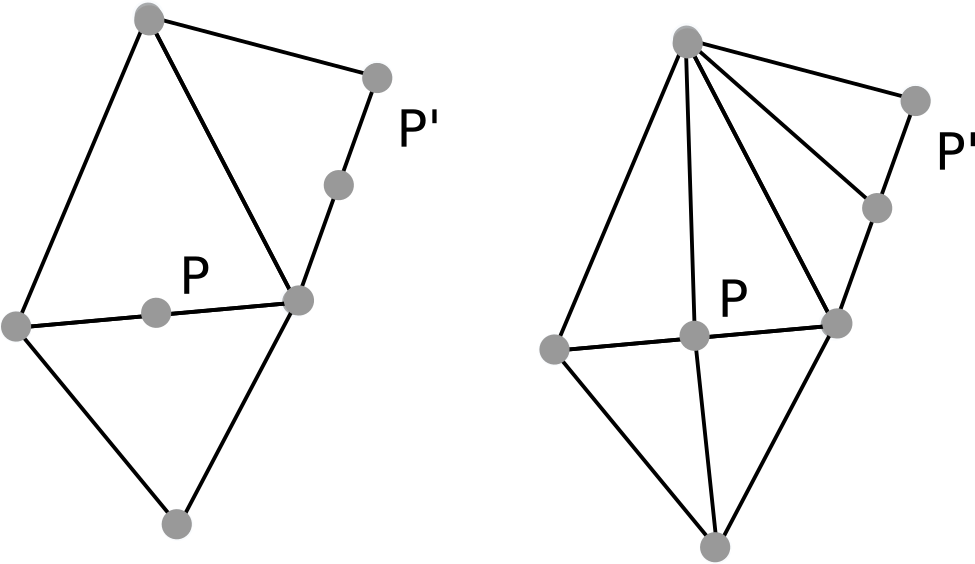
\includegraphics[scale=0.8]{adding2}
\end{figure}
  
  \onslide<3>
  
  \begin{figure}
\centering
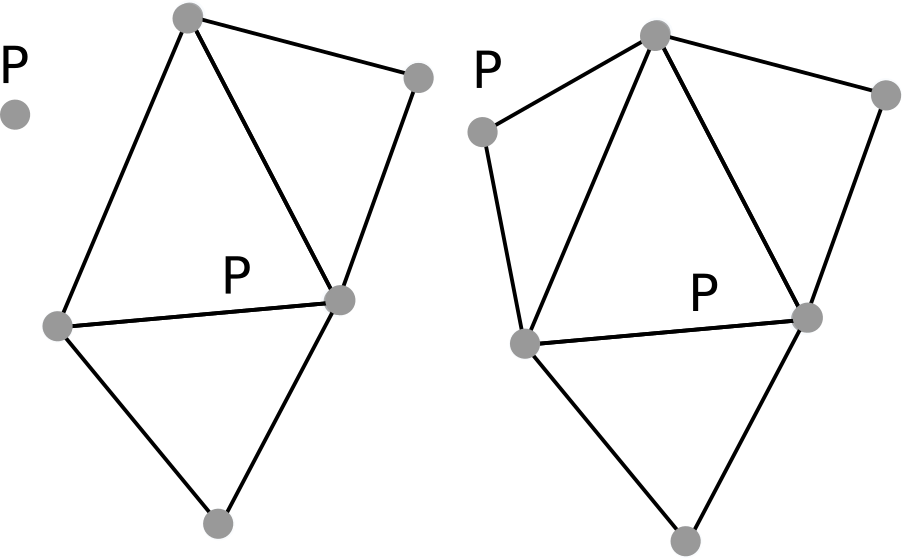
\includegraphics[scale=0.8]{adding3}
\end{figure}

\end{overprint}


\end{frame}


\subsection{Flipping Edges}
\begin{frame}{Transforming a triangulation into a Delaunay triangulation}

Obtain a Delaunay triangulation by repeating the same step: for each pair of triangles that does not meet the Delaunay condition, flip the common edge of the two triangles.

\begin{figure}
\centering

\includegraphics[scale=1]{dessin1}
\end{figure}
 
\end{frame}


\section{The Formalisation}


\subsection{Functions and Geometrical Predicates}



\begin{frame}{\tt in\_triangle}
 We need to define what it means to be in a triangle.

\begin{minipage}{.6\textwidth}
\begin{uncoverenv}<2->
   The notion of {\tt is\_left\_of} gives a nice, abstract way to do that.
 \end{uncoverenv}
   \end{minipage}%
  \begin{minipage}{.4\textwidth}
  \begin{overprint}
\onslide<2->

        \begin{figure}
  	\centering
 	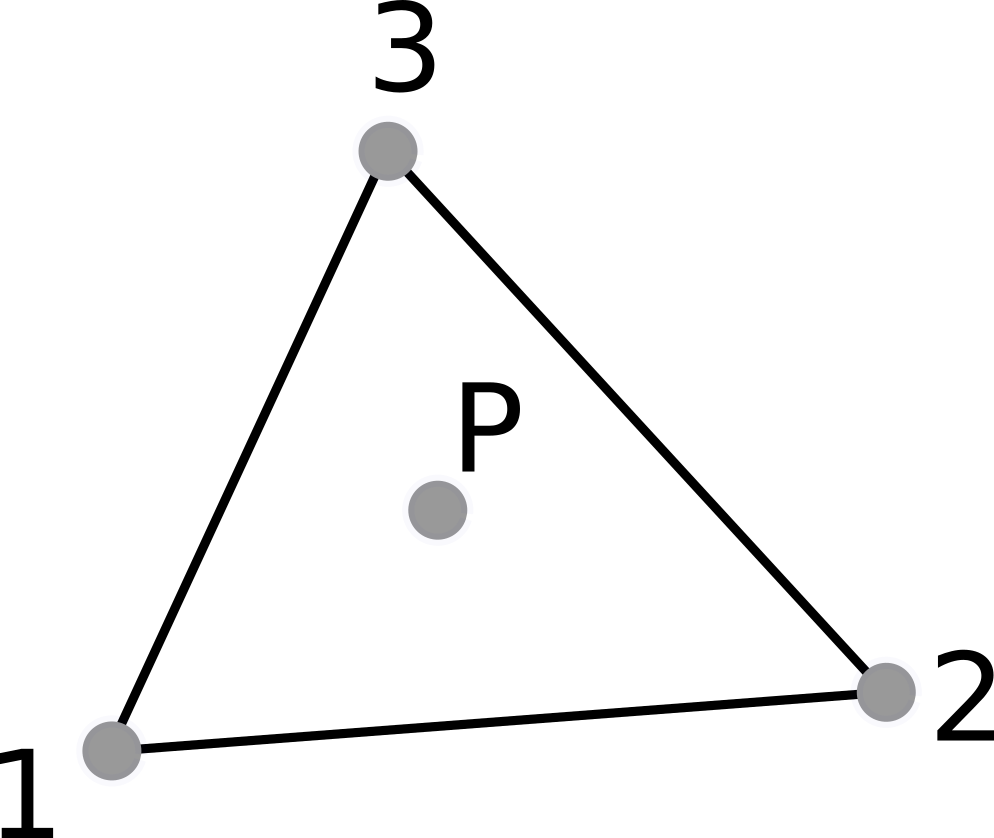
\includegraphics{intriangle}
      \end{figure}
  \end{overprint}
\end{minipage}
\begin{uncoverenv}<3>
 
 {\small \begin{tabular}{ll}
       {\tt in\_triangle t P = }& {\tt is\_left\_of (vertex1 t) (vertex2 t) P} $\wedge$\\
        &{\tt is\_left\_of P (vertex2 t) (vertex3 t)} $\wedge$\\
  & {\tt is\_left\_of (vertex1 t) P (vertex3 t)}
      \end{tabular}}

\end{uncoverenv}
\end{frame}



\begin{frame}{Requirements}
 
 We require in any instantiation of the formalisation:
 \begin{itemize}
  \item Some types for the basic concepts (triangles, points, ...).
  \item Some functions ({\tt vertices\_to\_triangle}, ...).
  \item Some geometrical predicates.
 \end{itemize}
 \begin{uncoverenv}<2->
 Geometrical predicates include:
 \end{uncoverenv}
\vspace{0.15cm}

\begin{minipage}{.6\textwidth}
 \begin{itemize}
  \item<2-> {\tt is\_left\_of A B C},
  \item<3-> {\tt is\_on\_line A B C},
  \item<4-> {\tt is\_left\_or\_on\_line A B C}
  \item<5-> (...)
  \end{itemize}
\end{minipage}%
\begin{minipage}{.4\textwidth}
  \begin{overprint}
   \onslide<2>
     \begin{figure}
   \centering
  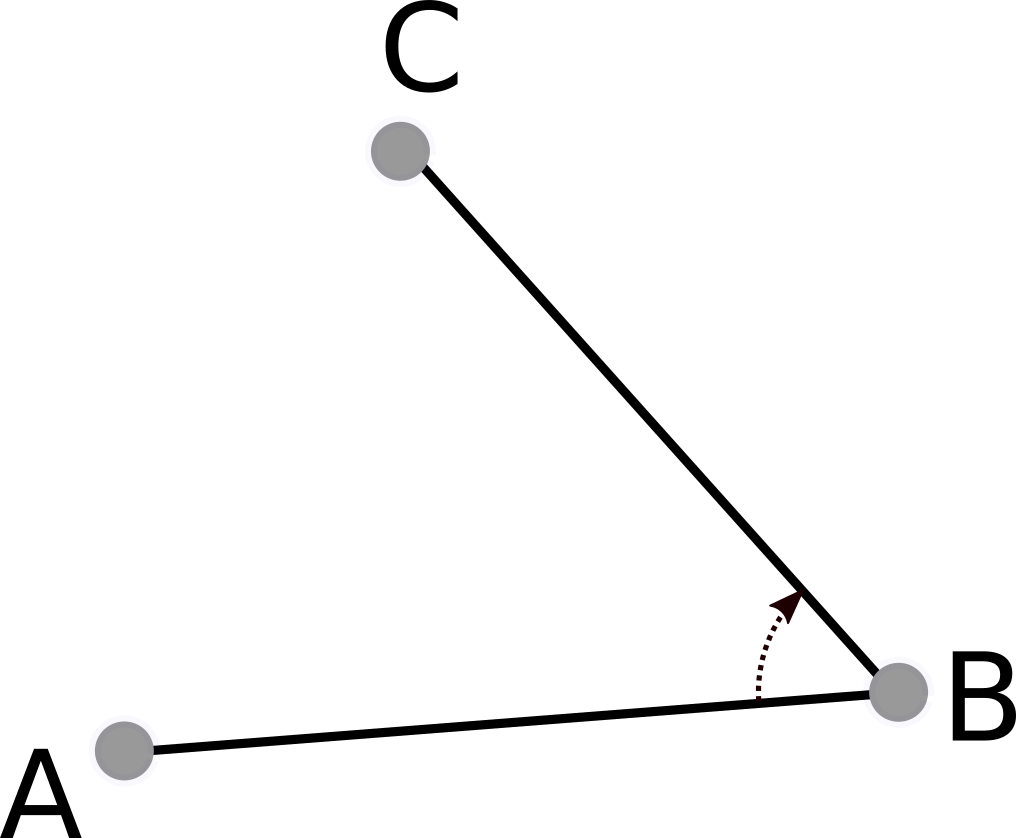
\includegraphics[scale=1.3]{isleftof}
 \end{figure}  
 
   \onslide<3>
   \vspace{0.3cm}
     \begin{figure}
   \centering
  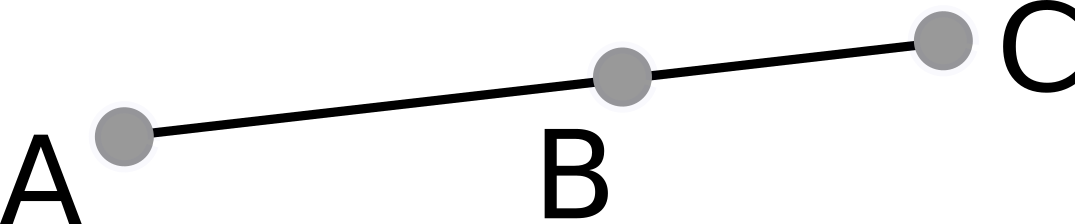
\includegraphics[scale=1.3]{isonline}
 \end{figure}  
 
   \onslide<4->
     \begin{figure}
   \centering
  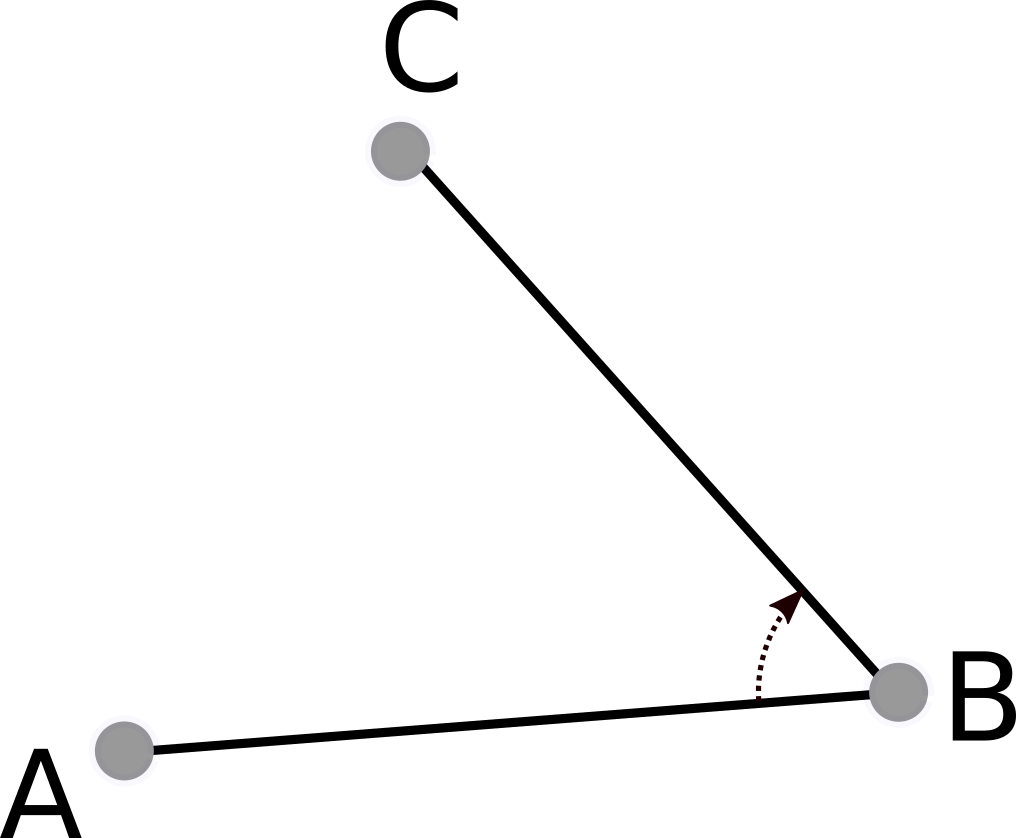
\includegraphics[scale=1.3]{isleftof}
 \end{figure}  
 
  \end{overprint}
\end{minipage}

\end{frame}

\begin{frame}{\tt oriented\_surface}
We derive three of those predicates from a function, {\tt oriented\_surface}:
{\small   \begin{itemize}
\item<2-> {\tt is\_left\_of A B C := oriented\_surface A B C > 0}.
  \item<3-> {\tt is\_on\_line A B C := oriented\_surface A B C = 0}.
  \item<4-> {\tt is\_left\_or\_on\_line A B C := oriented\_surface A B C $\geq$ 0}.

 \end{itemize} }


  \begin{figure}
  \centering
  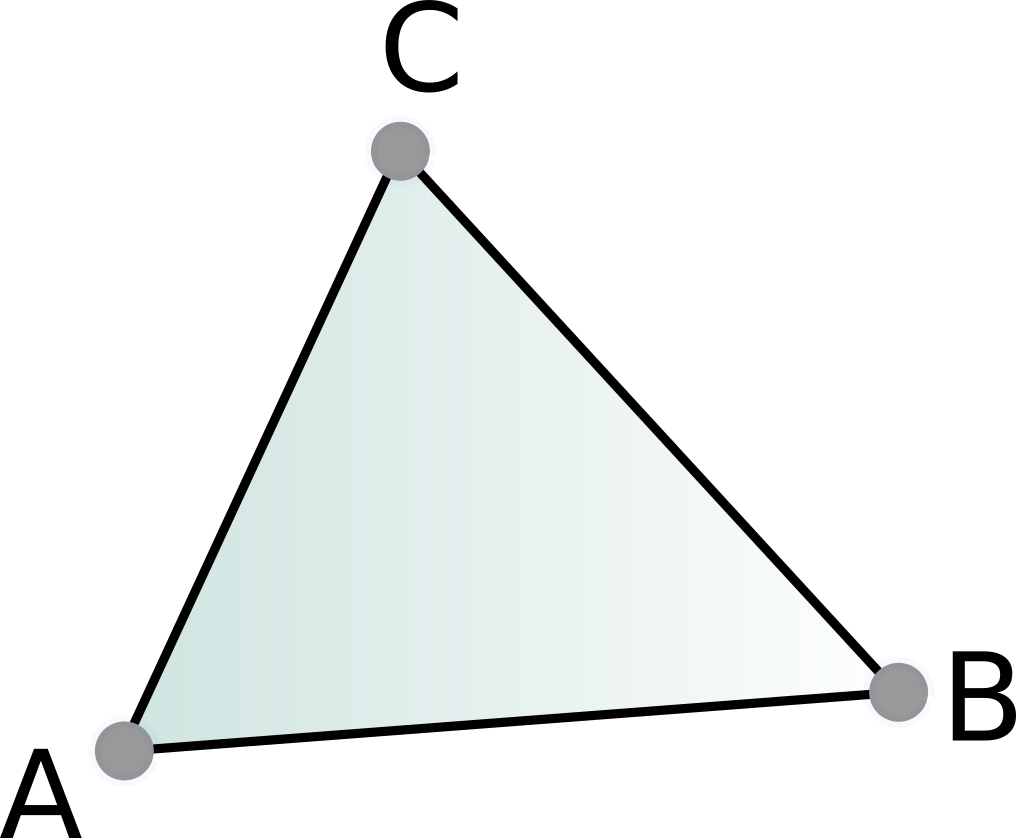
\includegraphics[scale=1]{Surface}
  \caption{\label{surface} Here, {\tt ABC} has a positive oriented surface whereas {\tt ACB} has a negative oriented surface.}
\end{figure}


\end{frame}


\subsection{Hypotheses}

\begin{frame}{Hypotheses}
 We put assumptions on these functions and predicates. For instance:
 \begin{itemize}
  \item<1-> The oriented surface of a segment should be 0.
  \item<2-> The oriented surface of {\tt CAB} is the same as {\tt ABC}.
  \item<3-> The vertices of the triangle created by {\tt vertices\_to\_triangle A B C} should be  {\tt A}, {\tt B} and {\tt C}.
 \end{itemize}

\end{frame}


\subsection{Geometrical Properties}

\begin{frame}{Definition of a triangulation}

 A triangulation {\tt Tr} on a data set {\tt D} is a finite set of triangles with points of {\tt D} as vertices which satisfies the following properties:
\begin{enumerate}
\item<2-> {\tt covers\_hull}  \tikzmark{start}
\item<2-> {\tt covers\_vertices} \tikzmark{end}
\item<3-> {\tt no\_cover\_intersection}\tikzmark{start2}
\item<3-> {\tt no\_point\_on\_segment \hspace{0.2 cm}}\tikzmark{end2}
\item<4-> {\tt triangle\_3\_vertices}\tikzmark{start3}
\item<4-> {\tt triangle\_nempty}
\item<4-> {\tt oriented\_triangle\_triangulation} \tikzmark{end3}
\end{enumerate}
\begin{uncoverenv}<2->
\begin{tikzpicture}[remember picture,overlay]
\draw[decorate,decoration={brace,raise=12pt}]
  ([yshift=2ex]{{pic cs:end}|-{pic cs:start}}) --
    node[xshift=15pt,anchor=west] {Tiling of the convex hull.} 
  ([yshift=-0.5ex]pic cs:end);
\end{tikzpicture}
\end{uncoverenv}

\begin{uncoverenv}<3->

\begin{tikzpicture}[remember picture,overlay]
\draw[decorate,decoration={brace,raise=12pt}]
  ([yshift=2ex]{{pic cs:end2}|-{pic cs:start2}}) --
    node[xshift=15pt,anchor=west] {Intersection of triangles.} 
  ([yshift=-0.5ex]pic cs:end2);
\end{tikzpicture}
\end{uncoverenv}

\begin{uncoverenv}<4->
\begin{tikzpicture}[remember picture,overlay]
\draw[decorate,decoration={brace,raise=12pt}]
  ([yshift=2ex]{{pic cs:end3}|-{pic cs:start3}}) --
    node[xshift=15pt,anchor=west] {No degenerate triangles.} 
  ([yshift=-0.5ex]pic cs:end3);
\end{tikzpicture}
\end{uncoverenv}

\end{frame}


\section{Operations and Proofs}
\subsection{Operations}
\begin{frame}{Operations: Adding points}
Two operations written. The first one is: given a triangle {\tt T} ({\tt ABC}), a point {\tt P} which is an interior point of {\tt T}, a triangulation {\tt Tr}, {\tt split\_triangle Tr T P}
returns {\tt (Tr $\smallsetminus$ T) $\cup$ $\{$ABP;PBC;APC$\}$}

\begin{figure} 
  \centering
  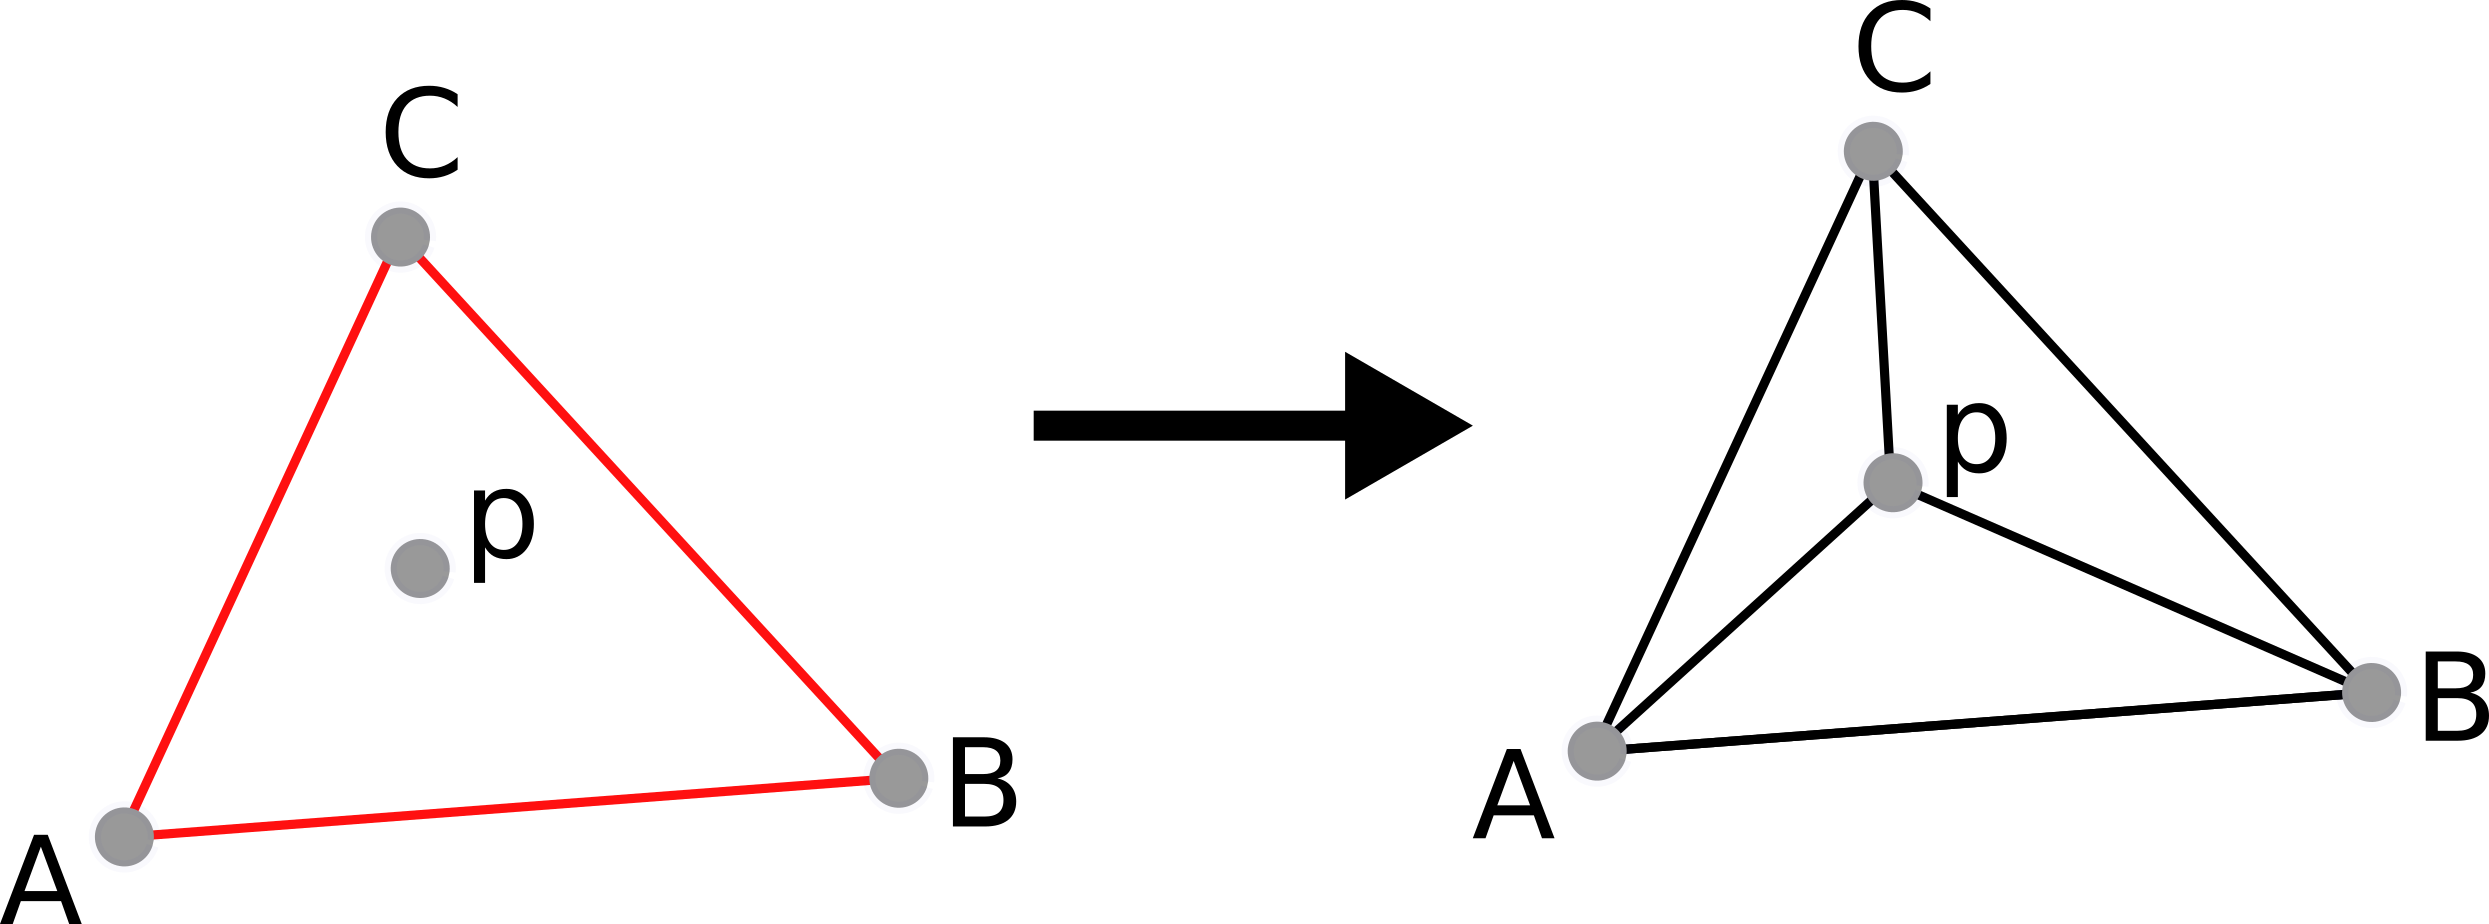
\includegraphics[scale=1.2]{split_triangle}
\end{figure}
  \end{frame}
 

  \begin{frame}{Operations: Flipping edges}
  
   The second one is: given {\tt T1} ({\tt ABC}) and {\tt T2} ({\tt ACD}), {\tt flip\_edge Tr T1 T2 A B C D} returns {\tt (Tr $\smallsetminus$ T1 $\smallsetminus$ T2) $\cup$ $\{$ABD;BCD$\}$}.
   

 \begin{figure}
  \centering
  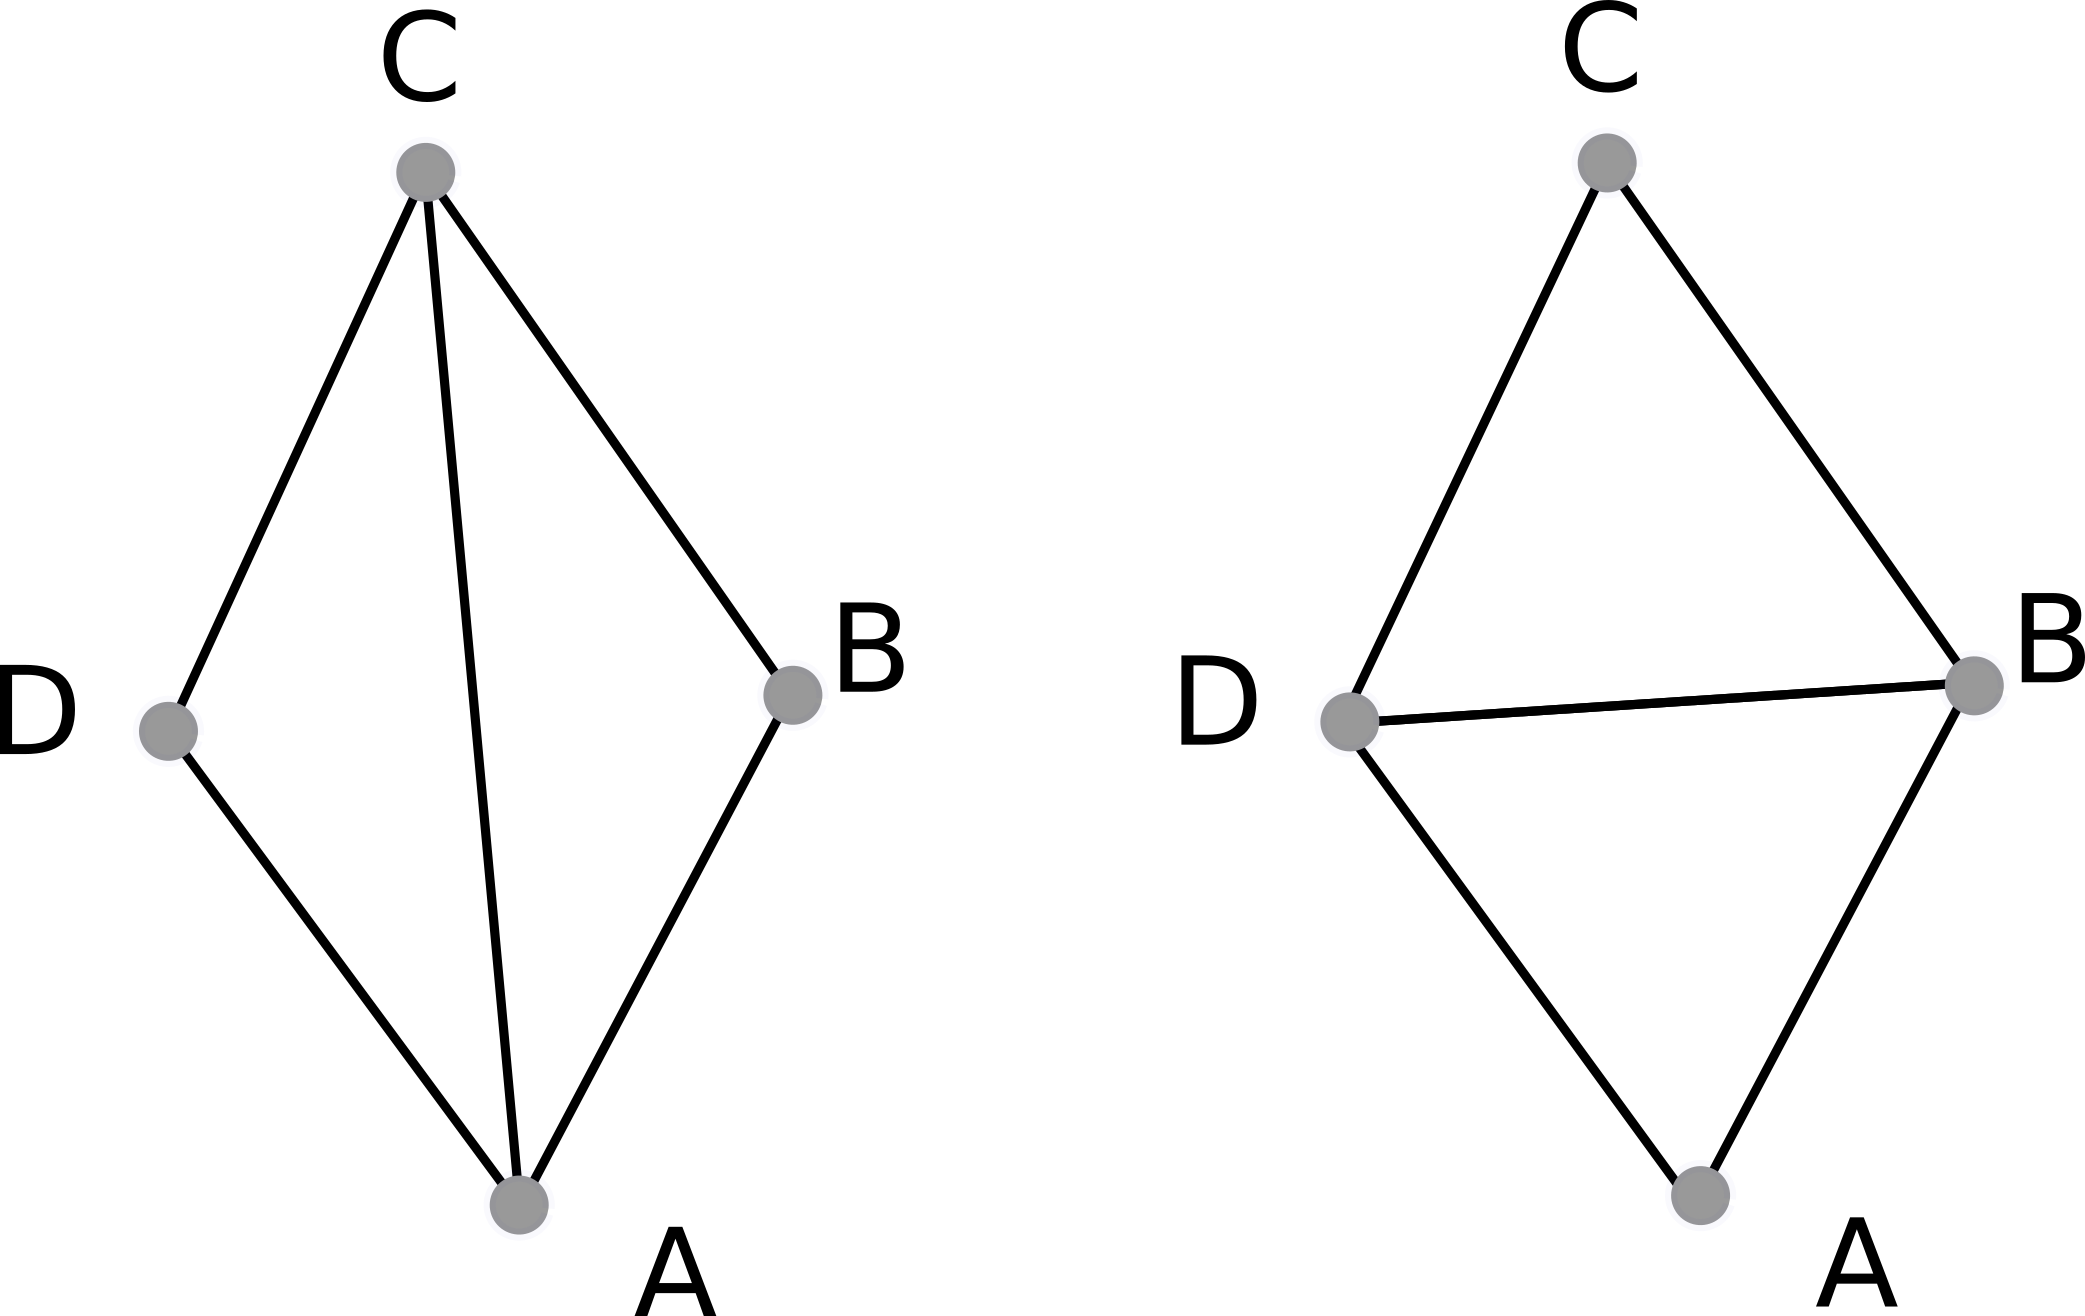
\includegraphics[scale=0.8]{flip_edge}

\end{figure}

\end{frame}

\subsection{Proofs}

\begin{frame}{Difficulties encountered}
Idea of the proofs: case-based reasonning, with some intermediary lemmas.

Some common difficulties:
\begin{itemize}
 \item<2-> Number of similar cases slowing down the proofs.
 \item<3-> Problems of symmetry ({\tt is\_left\_of A B C} vs {\tt is\_left\_of C A B}): a first try with {\tt easygeo}.
\end{itemize}

\begin{uncoverenv}<4->
$\rightarrow$ Symptoms of a more important problem: the lack of way to deal with the inherent symmetry of triangles.
\end{uncoverenv}


\end{frame}


\section{Conclusion}
\begin{frame}{Conclusion}
Work done:
\begin{itemize}
 \item Formalise in Coq the abstract concept of Delaunay triangulations.
 \item Prove some useful geometric lemmas.
 \item Write two operations that are part of an algorithm to compute Delaunay triangulations and prove their correctness.
 \item Write an instantiation of the abstracted concepts, with implementations for the functions and predicates and partially prove the correctness of this instantiation.
 \end{itemize}

\begin{uncoverenv}<2->
Possible improvements?
\begin{itemize}
 \item Finish the proofs.
 \item Find a better way to use the symmetry.
 \item Higher dimensions.
 \item Better algorithms.
\end{itemize}
\end{uncoverenv}

\end{frame}

\section*{Addendum}

\begin{frame}{CC Systems}

  \begin{definition}
  A CC (counter-clockwise) System is a ternary relation used to show the counter-clockwise ordering of triples of points $pqr$ in general position in the plane.
  
 \end{definition}

\end{frame}


\begin{frame}

 A CC system has to follow five axioms.
\begin{enumerate}
\item<1-> Cyclicity: $abc \rightarrow bca$.
\item<2-> Antisymmetry: $abc\rightarrow \neg bac$.
\item<3-> Nondegeneracy: $abc \vee bac$ since $a$ $b$ and $c$ can't be aligned.
\item<4-> Interiority: $abd \rightarrow bcd \rightarrow adc \rightarrow abc$.
\item<5-> Transitivity: $ abc \rightarrow abd \rightarrow abq \rightarrow cbd \rightarrow dbq \rightarrow cbq $.
\end{enumerate}

\begin{overprint}
\onslide<4>
\begin{figure}
  \centering
  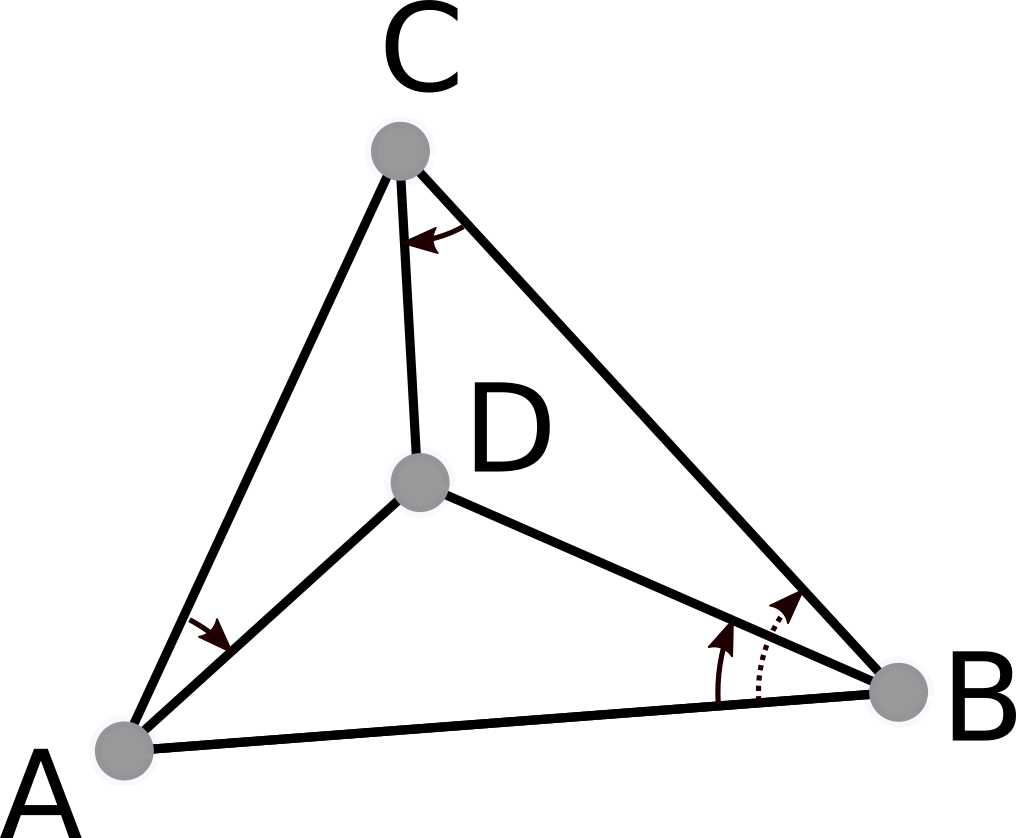
\includegraphics[scale=1.5]{Axiom4}

\end{figure}

\onslide<5>
\begin{figure}
  \centering
  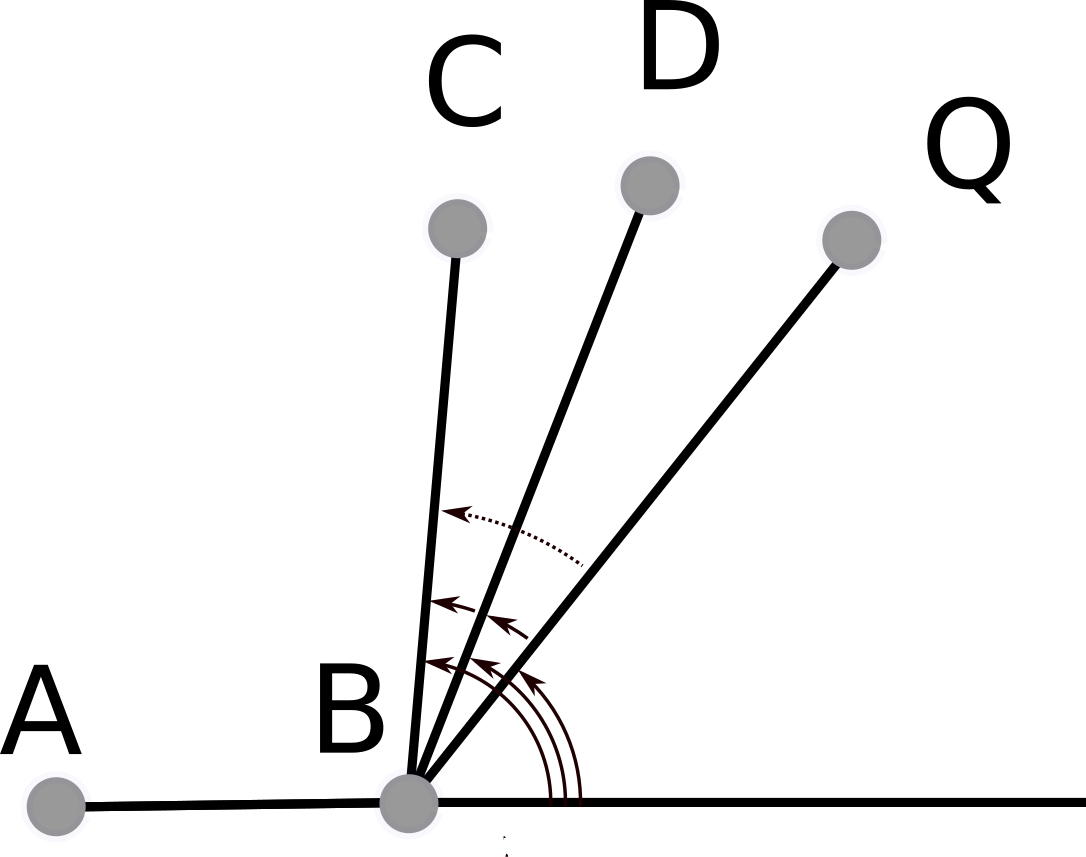
\includegraphics[scale=1.4 ]{Axiom5}

\end{figure}
\end{overprint}

\end{frame}

\end{document}
